\documentclass[tikz,border=10pt]{standalone}
% Coordinates: x = px*s, y = (629 - py)*s, s = 0.009445 (longest side = 8 cm)
\begin{document}
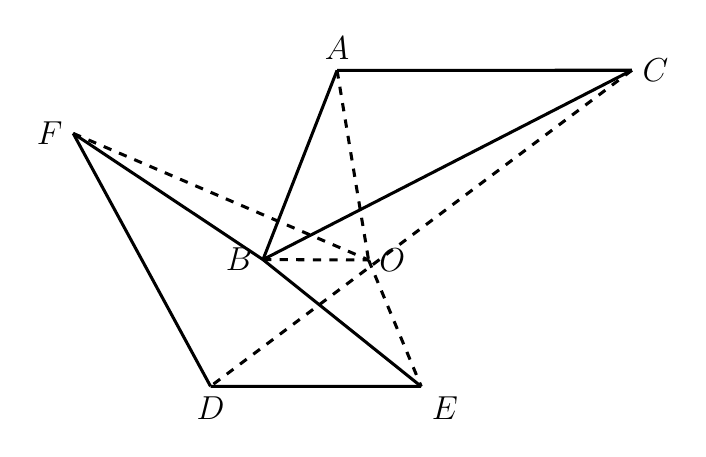
\begin{tikzpicture}[line width=1.1pt, line join=round, font=\fontsize{8.5}{10.2}\selectfont]
  % Named vertices (unchanged)
  \coordinate (A) at (4.342,4.986);
  \coordinate (C) at (8.086,4.987);
  \coordinate (F) at (0.991,4.185);
  \coordinate (B) at (3.401,2.582);
  \coordinate (O) at (4.742,2.578);
  \coordinate (D) at (2.735,0.973);
  \coordinate (E) at (5.411,0.971);

  % Solid edges
  \draw (A) -- (C);          % A-C
  \draw (A) -- (B);          % A-B
  \draw (B) -- (C);          % B-C
  \draw (F) -- (D);          % F-D
  \draw (D) -- (E);          % D-E
  \draw (F) -- (B) -- (E);   % F-B-E as one solid line

  % Dashed edges
  \draw[dashed] (A) -- (O);  % A-O
  \draw[dashed] (F) -- (O);  % F-O
  \draw[dashed] (C) -- (D);  % C-D, passes near O
  \draw[dashed] (B) -- (O);  % B-O
  \draw[dashed] (O) -- (E);  % O-E

  % Labels: larger size (\large) to match original; B moved to west of vertex
  \node[font=\large, above] at (A) {$A$};
  \node[font=\large, right] at (C) {$C$};
  \node[font=\large, left] at (F) {$F$};
  \node[font=\large, left] at (B) {$B$};
  \node[font=\large, right] at (O) {$O$};
  \node[font=\large, below] at (D) {$D$};
  \node[font=\large, below right] at (E) {$E$};
\end{tikzpicture}
\end{document}